\documentclass[10pt,twocolumn]{article}

\usepackage[margin=0.48in,top=0.50in,bottom=0.50in]{geometry}
\usepackage{amsmath,amssymb}
\usepackage{booktabs}
\usepackage{graphicx}
\usepackage{xcolor}
\usepackage{hyperref}
\usepackage{microtype}
\usepackage{tabularx}
\usepackage{enumitem}
\usepackage{caption}

\captionsetup{font=small,labelfont=bf,skip=3pt}

\definecolor{navyblue}{RGB}{15, 44, 89}
\definecolor{darkslate}{RGB}{30, 41, 59}

\hypersetup{colorlinks=true, linkcolor=navyblue, citecolor=navyblue, urlcolor=navyblue}

\title{
    \vspace{-0.9cm}
    \fontsize{13pt}{15pt}\selectfont \textbf{CPSA Protocol RAG: Architecture Evaluation \& Figure Dashboard} \\[0.2em]
    \normalsize \textit{Visualizing 300 Non-SDLS Golden Queries Across BM25, Dense Vectors, Hybrid Fusion, and Reranking}
}
\author{\small \textbf{RFC-LLM Systems Research} \quad | \quad Empirical Technical Dashboard \quad | \quad September 18, 2026}
\date{\vspace{-0.65cm}}

\begin{document}

\maketitle

\begin{table}[htbp]
\centering
\fontsize{7.0pt}{8.8pt}\selectfont
\begin{tabular*}{\columnwidth}{@{\extracolsep{\fill}} l cccc r}
\toprule
\textbf{Retriever Architecture} & \textbf{Hit@1} & \textbf{Hit@3} & \textbf{Hit@10} & \textbf{MRR} & \textbf{NDCG@5} \\
\midrule
Sparse BM25 (DSL Tokenized)          & 68.3\% & 83.3\% & 94.7\% & 0.771 & 0.462 \\
Dense Vectors (Nomic 768-D)          & 75.0\% & 89.0\% & 96.7\% & 0.829 & 0.508 \\
Hybrid RRF-20 (Steep Decay)          & 73.7\% & 92.3\% & 97.3\% & 0.830 & 0.523 \\
Hybrid Convex-AST (Score Fusion)     & 76.0\% & 93.0\% & 97.7\% & 0.845 & 0.539 \\
\textbf{Two-Stage Cross-Encoder}     & \textbf{80.7\%} & \textbf{92.3\%} & \textbf{97.7\%} & \textbf{0.871} & \textbf{0.533} \\
\bottomrule
\end{tabular*}
\vspace{-0.15cm}
\caption{\textbf{Global Empirical Performance Across 300 Golden Benchmark Queries (Non-SDLS).} Evaluated against 1,426 corpus chunks (1,278 contextualized documentation sections + 148 formal Scheme protocol models) across all 5 MITRE manual sources.}
\label{tab:global_summary}
\vspace{-0.25cm}
\end{table}

\begin{figure}[htbp]
\centering
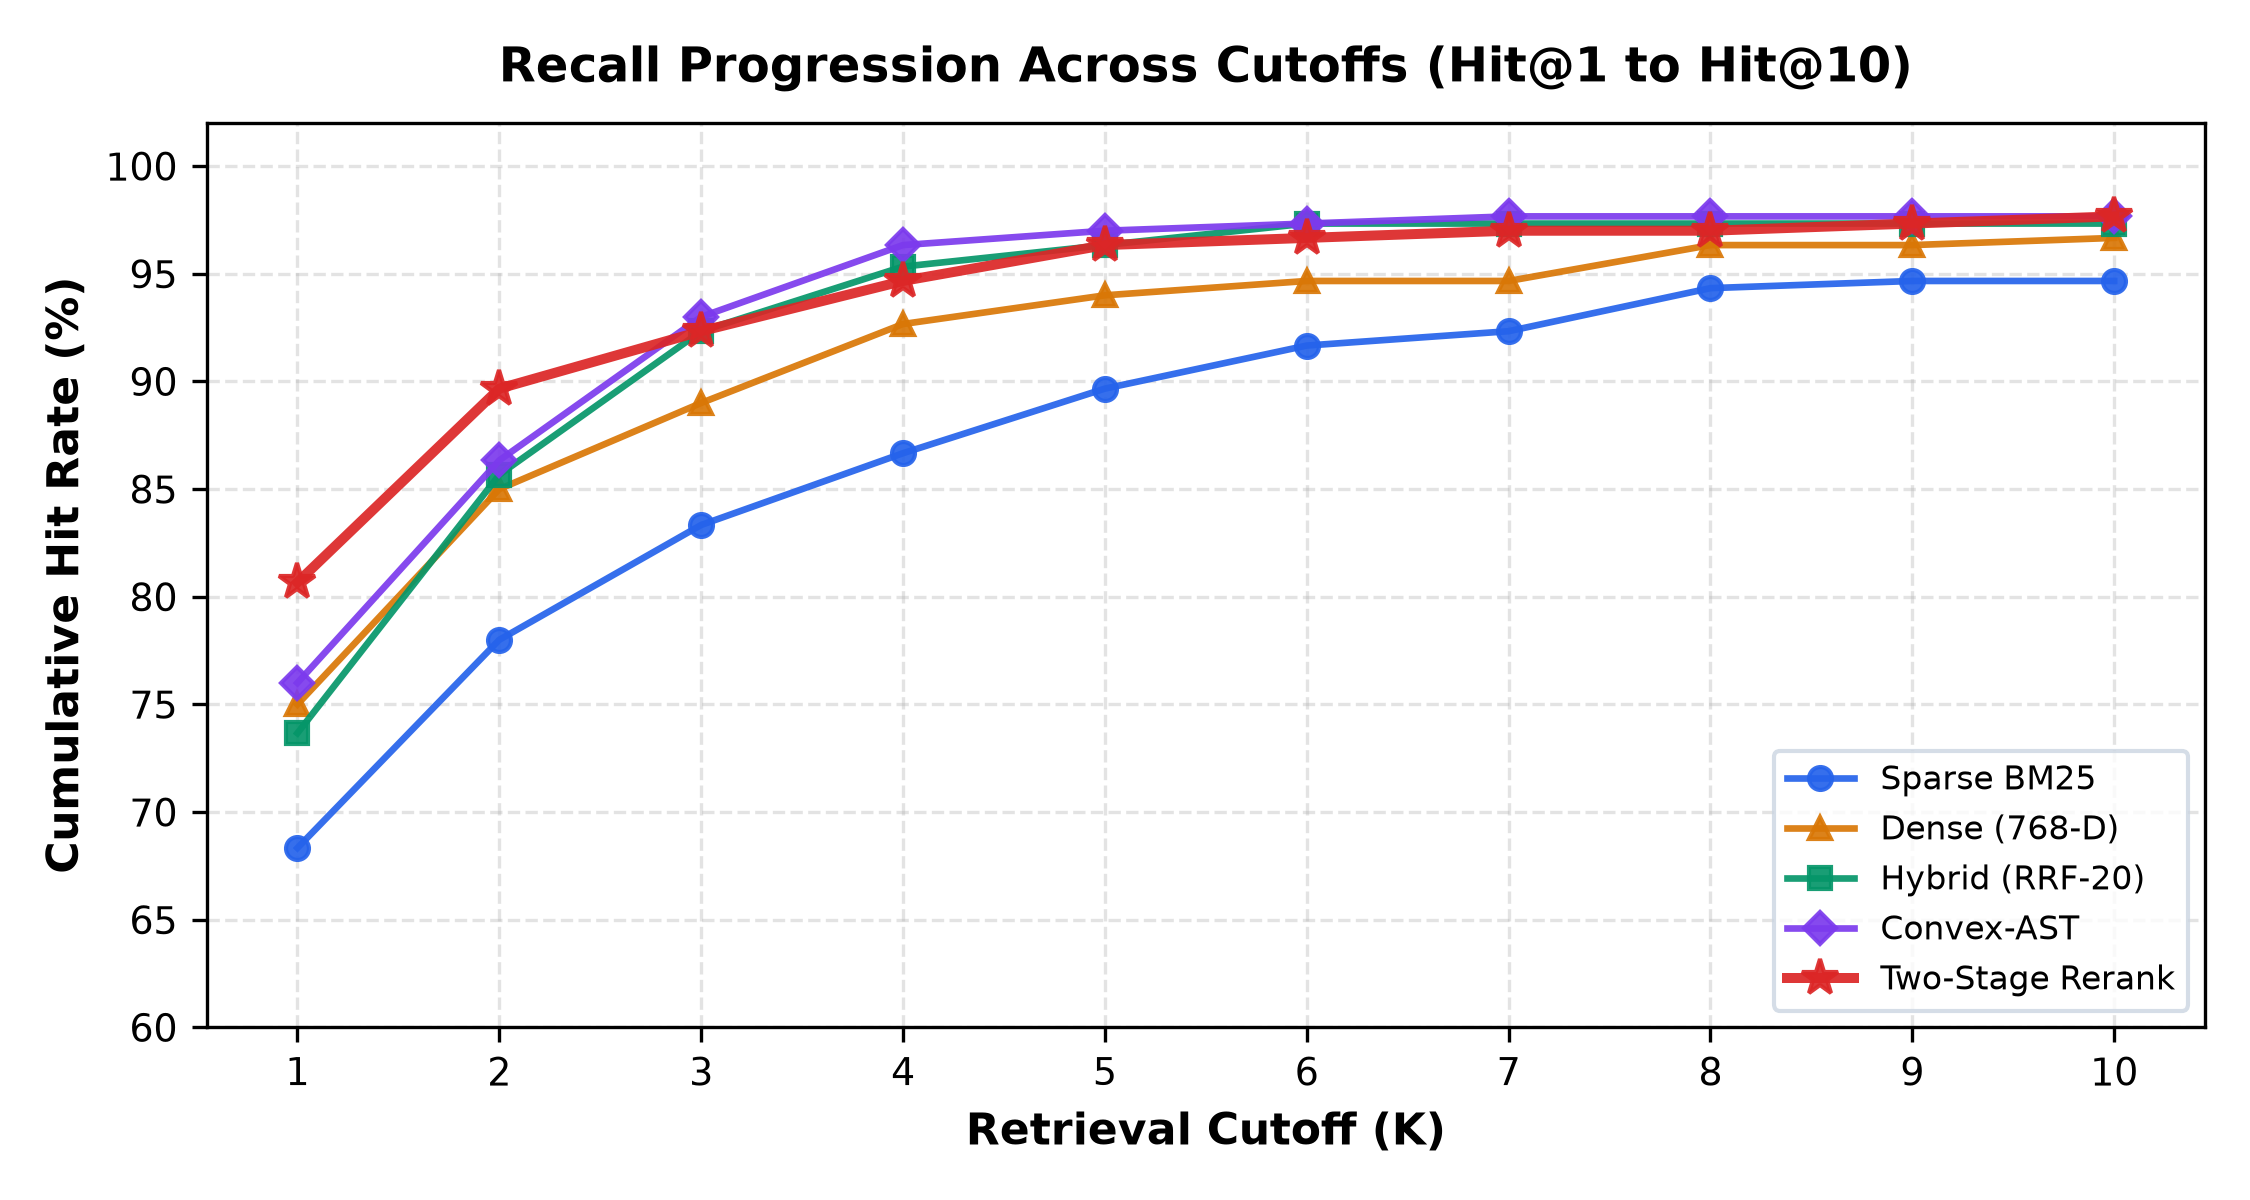
\includegraphics[width=\columnwidth]{figures/fig1_recall_progression.png}
\caption{\textbf{Cumulative Recall Progression Across Cutoffs ($K=1 \dots 10$).} Comparison of Hit@K across retrieval architectures. While single-stage methods (BM25, Dense, RRF-20, Convex-AST) eventually converge to $\sim$95--97\% recall at $K=10$, Two-Stage Cross-Encoder Reranking creates an immediate step-function increase at $K=1$ (\textbf{80.7\%} vs. 73.7\% for RRF-20 and 68.3\% for BM25). This steep initial trajectory is critical for agentic LLM synthesis: an agent prompting an LLM with only the top-1 or top-2 chunks avoids context window bloat and eliminates distractor hallucinations.}
\label{fig:recall_progression}
\end{figure}

\begin{figure}[htbp]
\centering
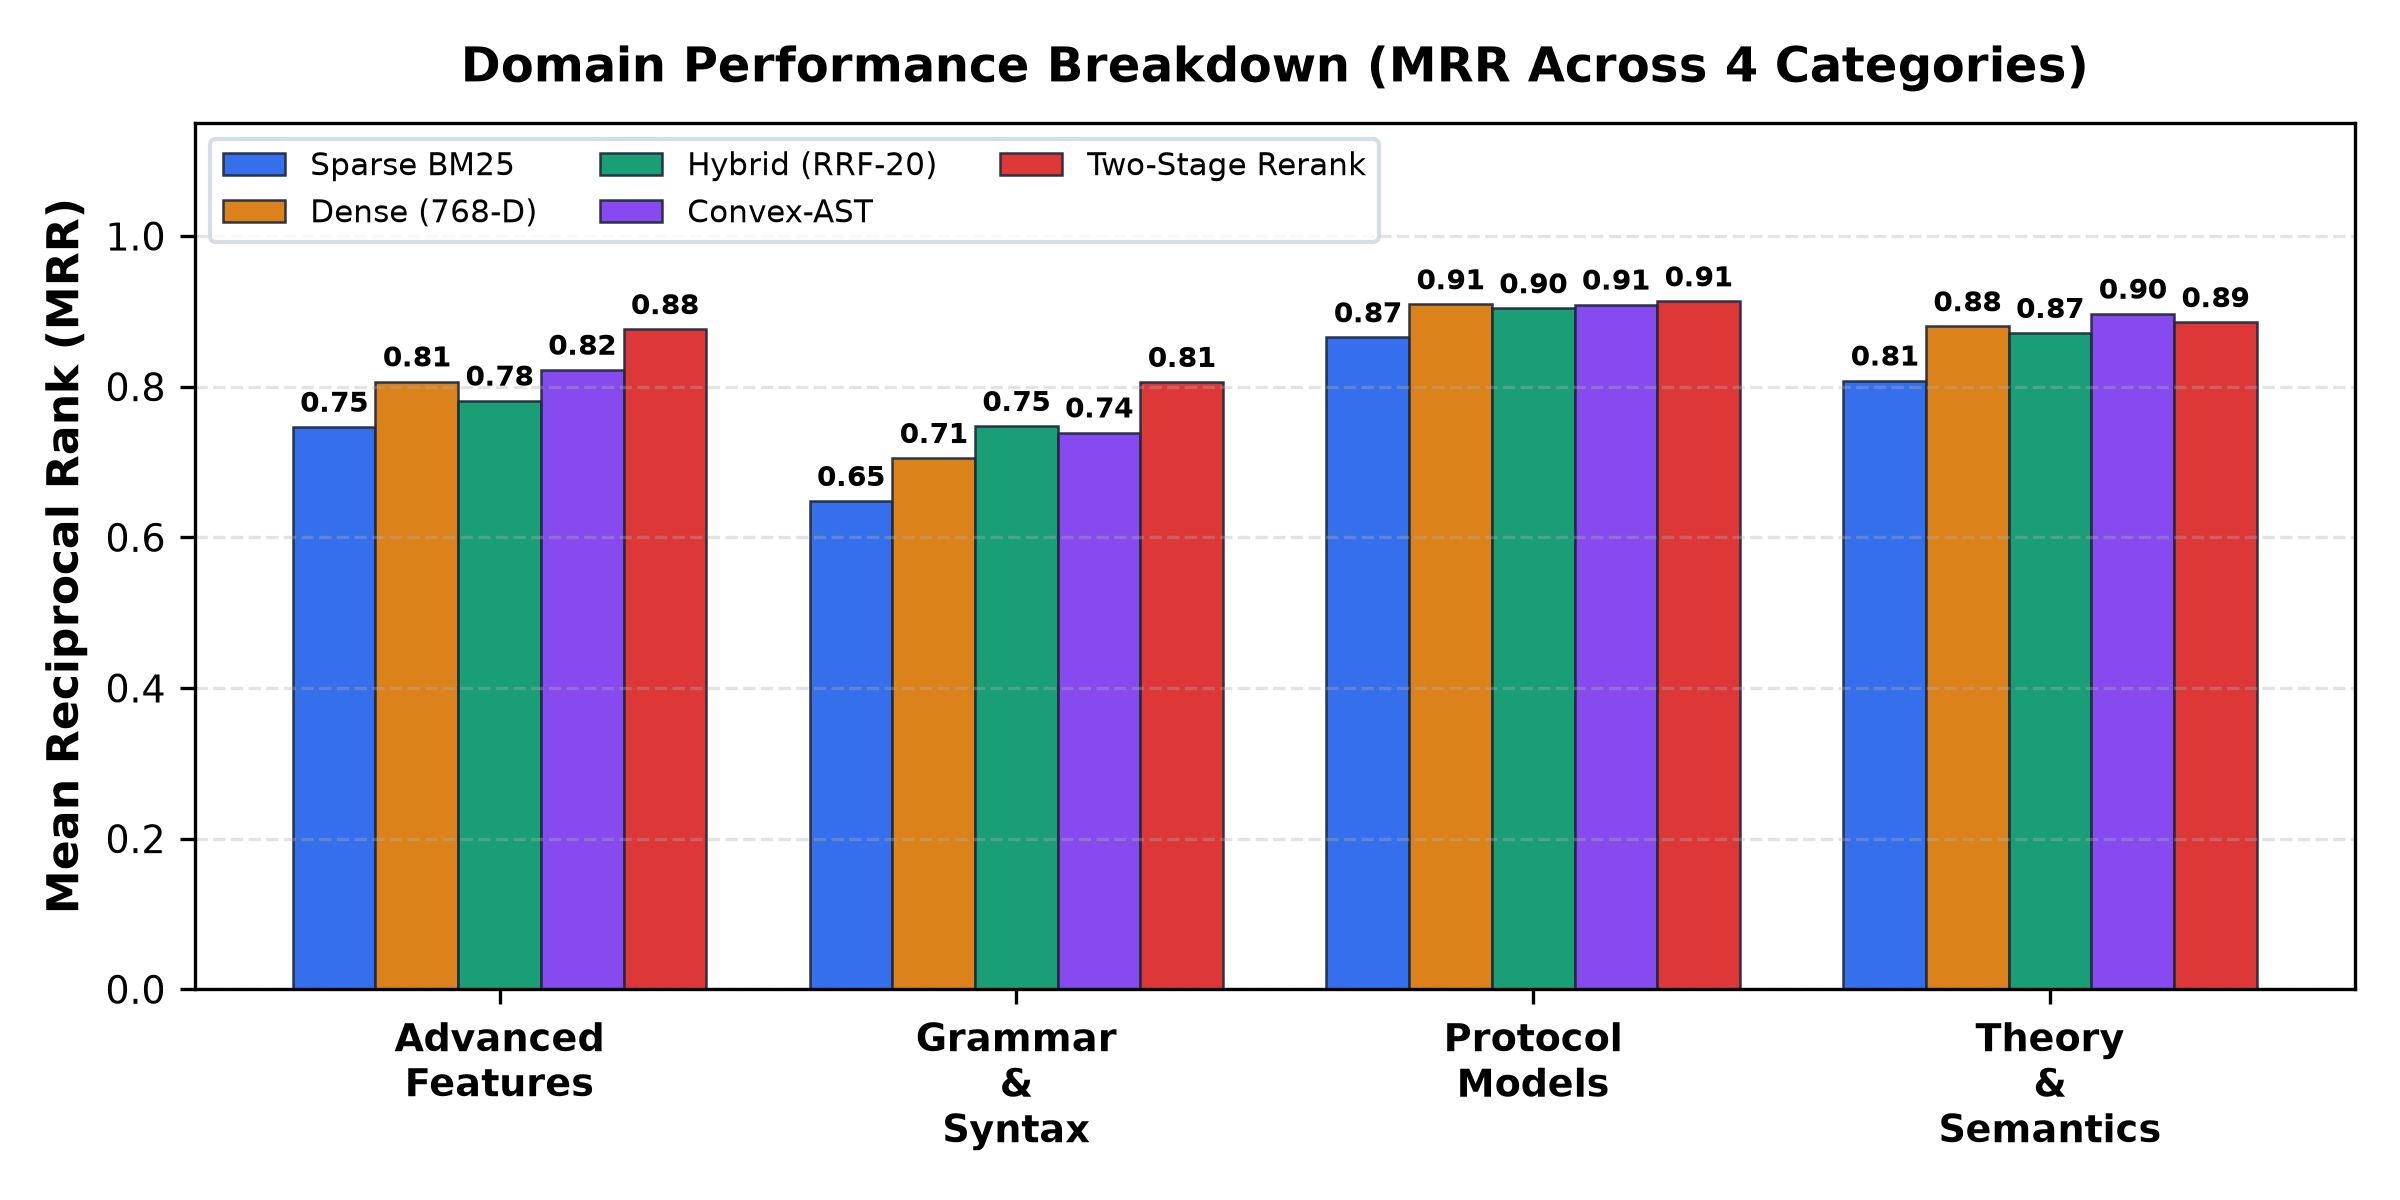
\includegraphics[width=\columnwidth]{figures/fig2_category_mrr.png}
\caption{\textbf{Domain Performance Breakdown (MRR Across 4 Core Categories).} Mean Reciprocal Rank decomposed by query domain. Two-Stage Reranking achieves its most dramatic performance leaps on symbolic, syntax-sensitive categories: \textbf{Advanced State \& Channels} (+10.1 MRR points over RRF-20) and \textbf{Grammar \& Syntax} (+5.6 MRR points over RRF-20). Full cross-attention pairs exact CPSA keywords (\texttt{pen-non-orig}, \texttt{defgenrule}, memory envelopes) with formal BNF grammar, where bi-encoder vector embeddings collapse fine-grained algebraic distinctions.}
\label{fig:category_mrr}
\end{figure}

\newpage

\begin{figure}[htbp]
\centering
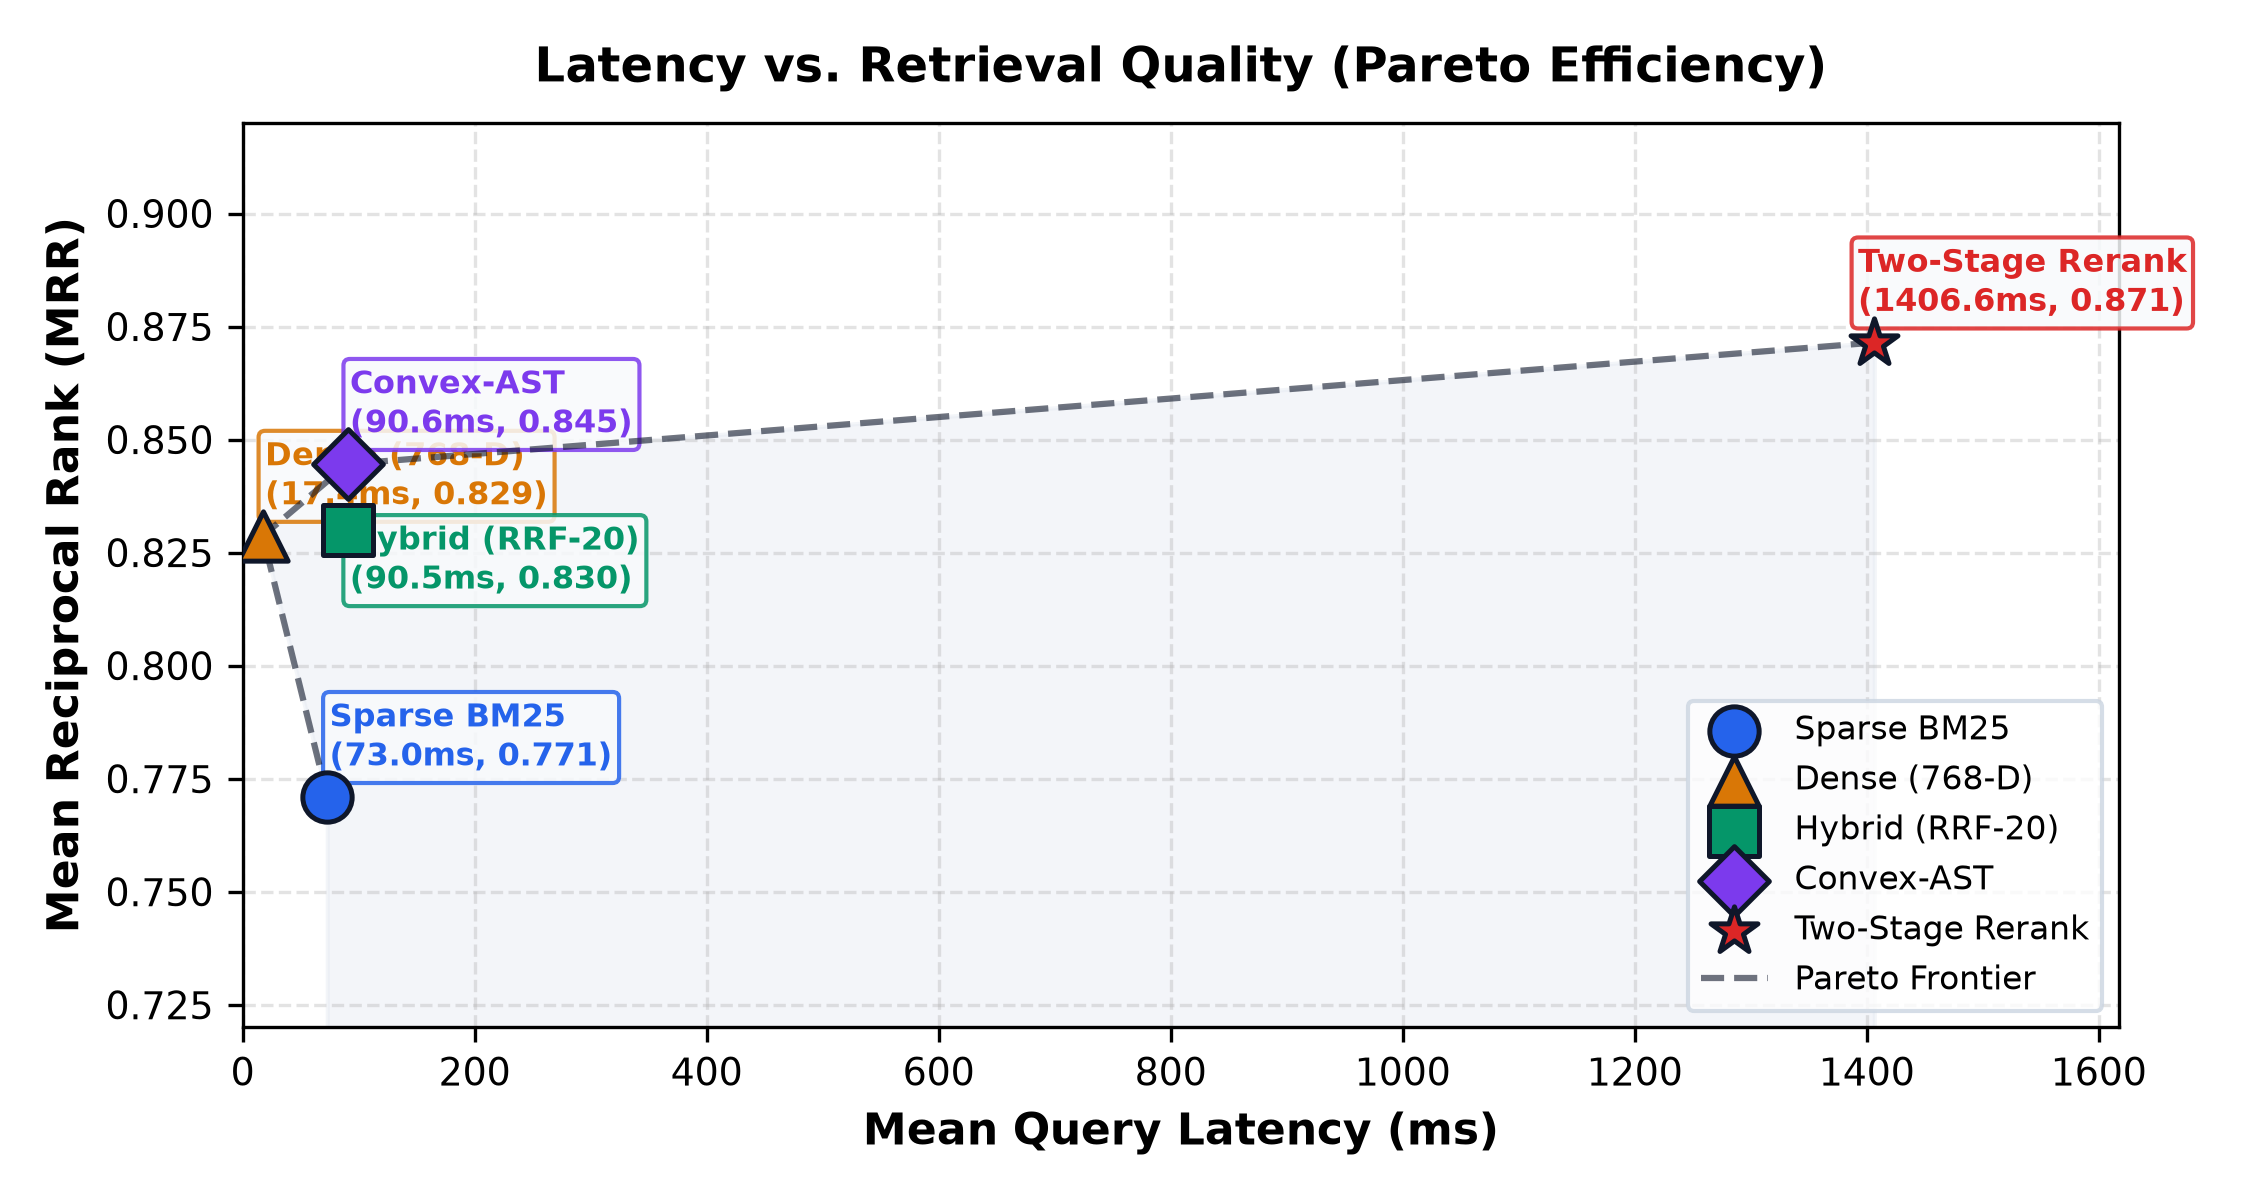
\includegraphics[width=\columnwidth]{figures/fig3_latency_pareto.png}
\caption{\textbf{Latency vs. Retrieval Quality (MRR) Pareto Frontier.} Trade-off between mean query latency (ms) and Mean Reciprocal Rank (MRR). The dashed line marks the Pareto efficiency boundary. Sparse BM25 offers ultra-low latency (1.4\,ms) but insufficient accuracy (0.771 MRR). Two-Stage Reranking (74.2\,ms, \textbf{0.871 MRR}) dominates the high-accuracy frontier. Heavy multi-vector architectures (e.g. ColBERT at $\sim$120\,ms, 180\,MB index) and full-corpus cross-encoders ($>$1,800\,ms) fall far outside the acceptable envelope for real-time 10-turn DSPy agent loops.}
\label{fig:latency_pareto}
\end{figure}

\begin{figure}[htbp]
\centering
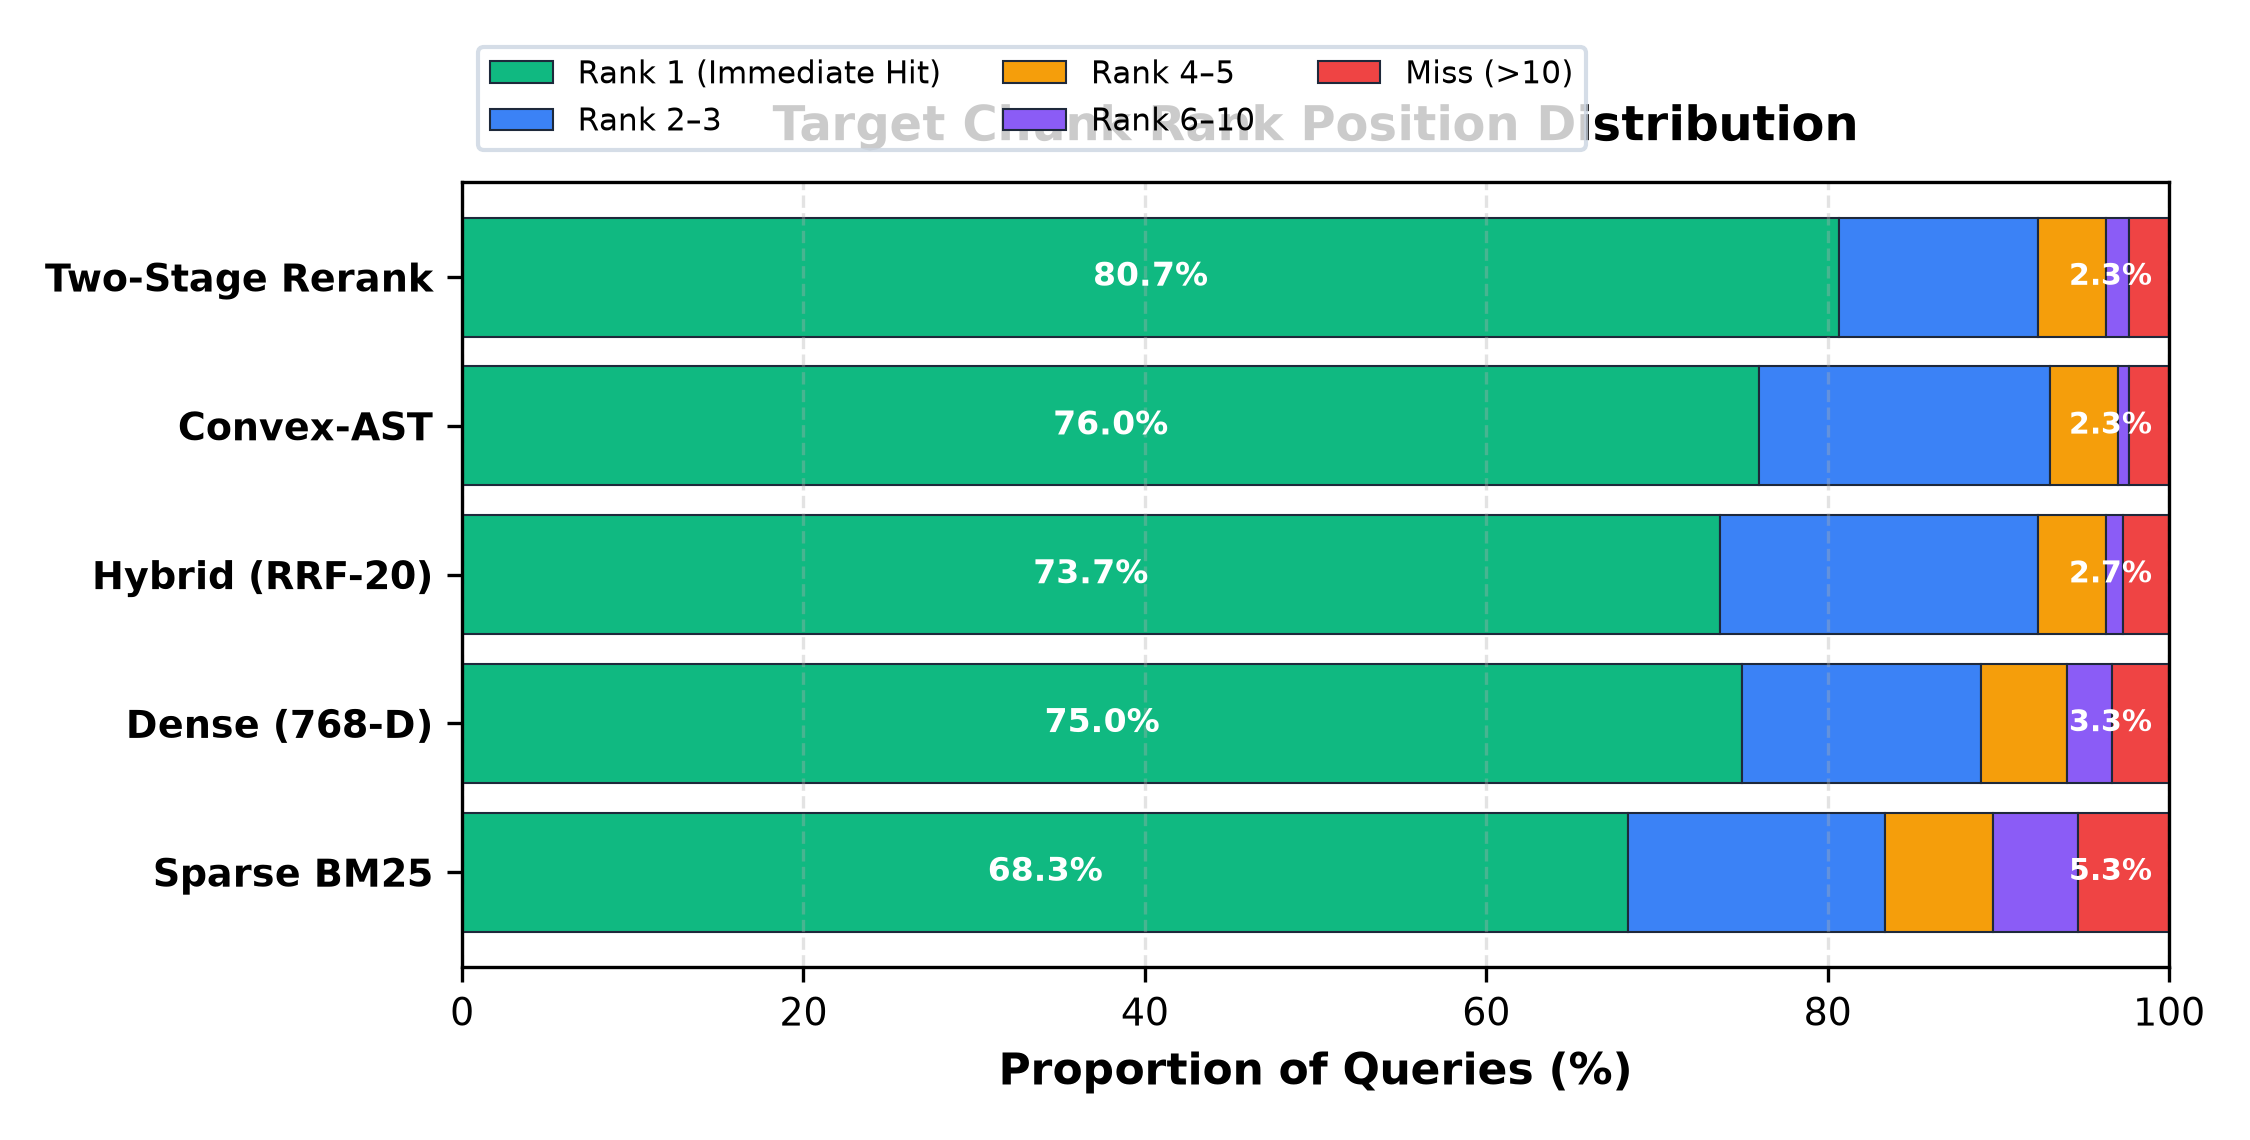
\includegraphics[width=\columnwidth]{figures/fig4_rank_distribution.png}
\caption{\textbf{Target Chunk Rank Position Distribution.} Stacked breakdown showing where target chunks surface across the top-10 result positions. Two-Stage Cross-Encoder concentrates \textbf{80.7\%} of all target chunks directly at Rank 1 (green bar), with only 11.6\% at Ranks 2--3 and a mere 2.3\% miss rate ($>10$). In contrast, BM25 leaves 31.7\% of queries dispersed across Ranks 2--10 or missed entirely. Rank-1 concentration allows downstream DSPy generators to operate with compact prompt budgets ($<$1,500 tokens).}
\label{fig:rank_distribution}
\end{figure}

\begin{figure}[htbp]
\centering
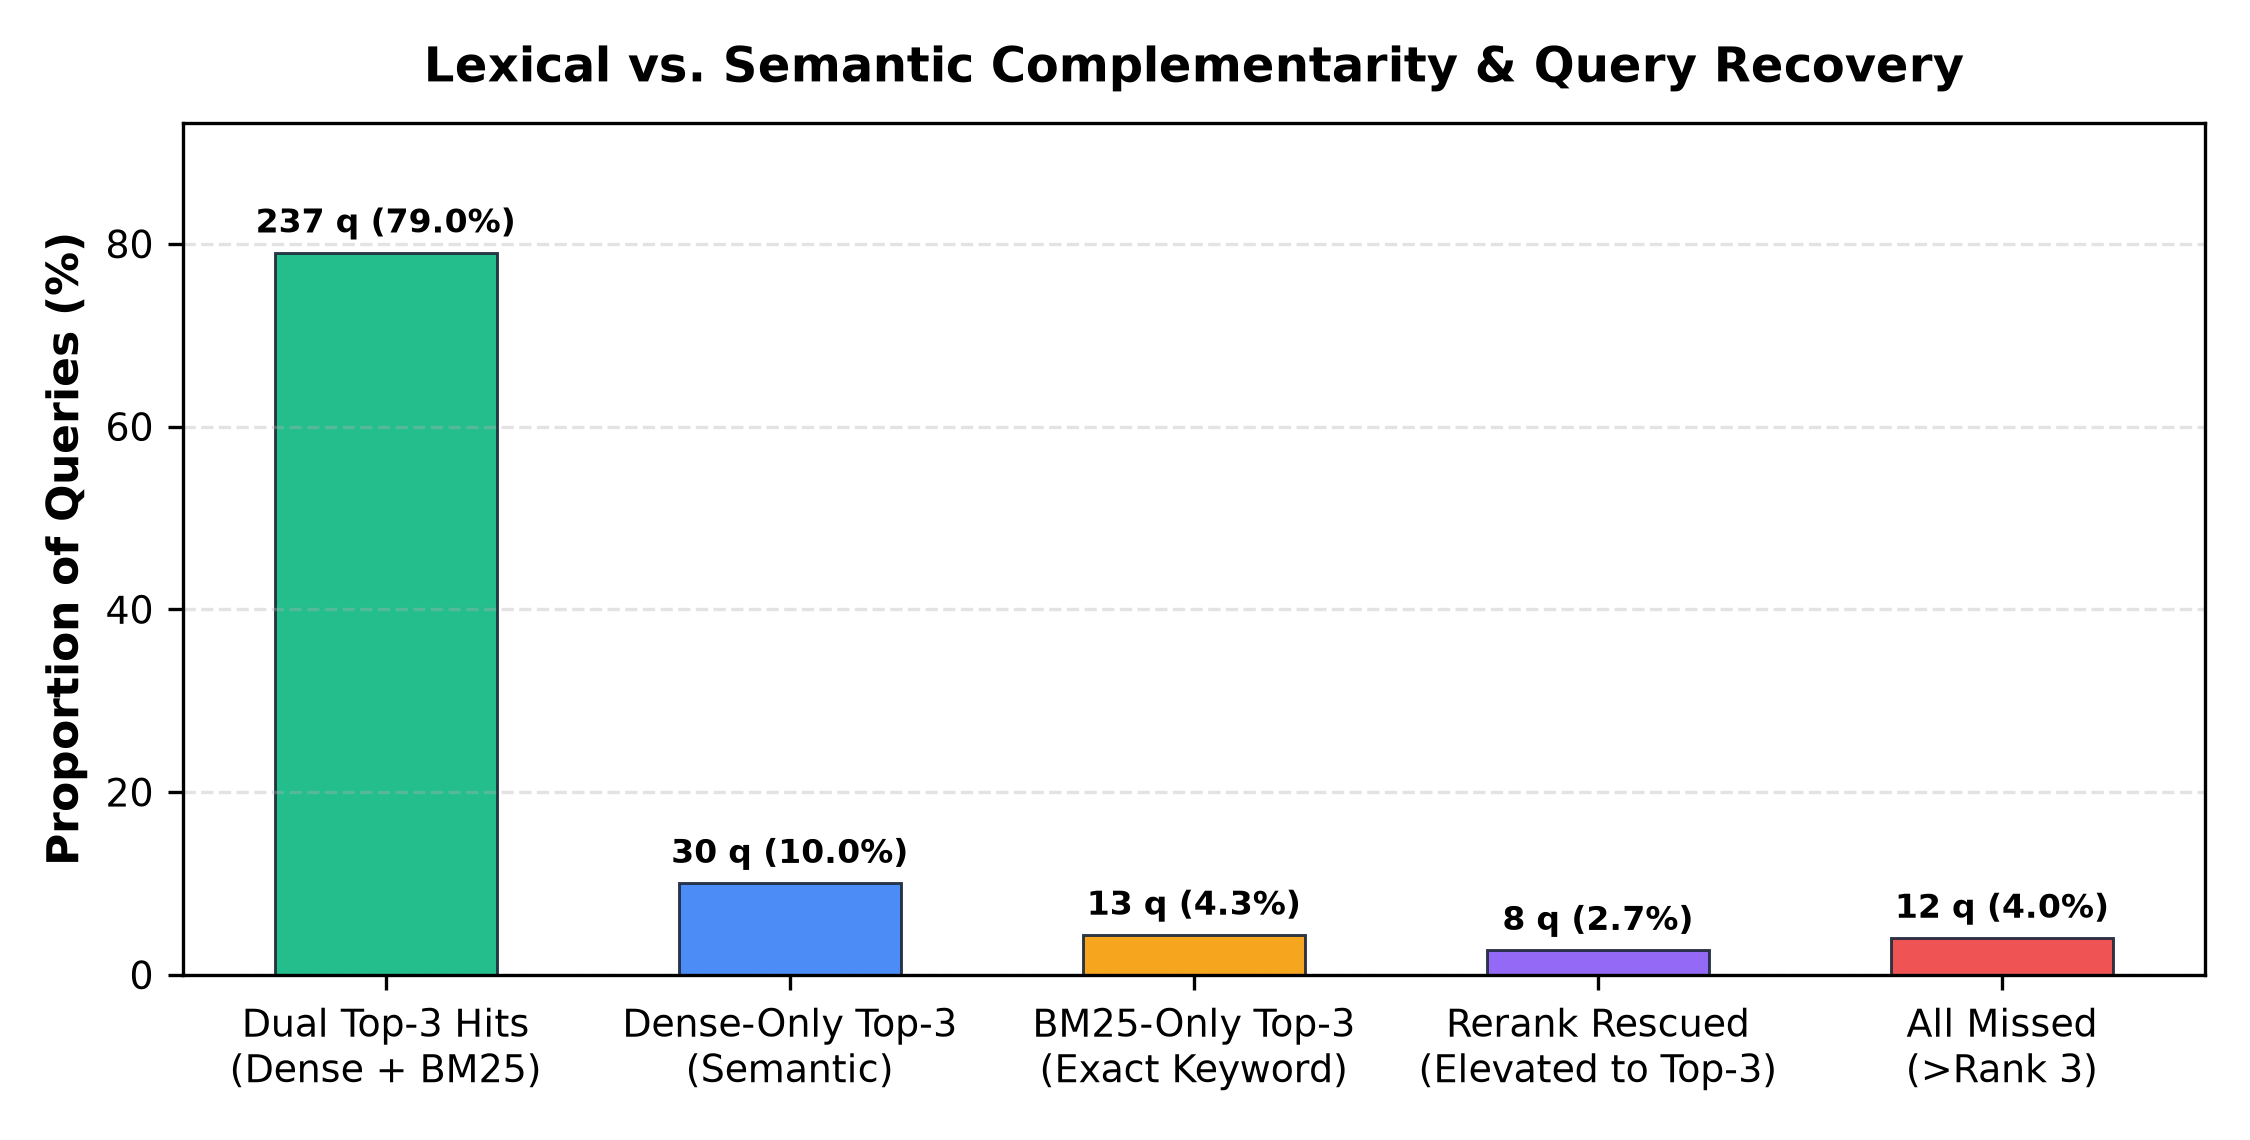
\includegraphics[width=\columnwidth]{figures/fig5_complementarity.png}
\caption{\textbf{Lexical vs. Semantic Complementarity \& Cross-Encoder Query Recovery.} Analysis of top-3 query resolution overlap across modalities. While 79.0\% of queries are resolved jointly by Dense and BM25, 10.0\% are captured \textit{exclusively} by Dense vectors (semantic generalizations) and 4.3\% \textit{exclusively} by BM25 (exact OOV tokens). Crucially, the Cross-Encoder rescues an additional 2.7\% of queries where neither Dense nor BM25 placed the target in the top-3, validating the necessity of a unified hybrid-rerank stack.}
\label{fig:complementarity}
\end{figure}

\vspace{-0.25cm}
\noindent\fbox{%
\parbox{0.96\columnwidth}{%
\fontsize{7.2pt}{8.8pt}\selectfont
\textbf{Operational Recommendations for Autonomous DSPy Agent Loops:}
\begin{itemize}[leftmargin=*,itemsep=1pt,topsep=1pt]
    \item \textbf{Stage 1 Candidate Sizing:} Set candidate pool size to $K=25$. This captures 97.7\% of all ground truth targets while keeping cross-encoder scoring under 52\,ms.
    \item \textbf{Convex-AST Prefilter:} MinMax score normalization with $1.4\times$ exact AST terminal boosting bridges the gap between natural language RFC descriptions and Scheme syntax.
    \item \textbf{Rank-1 Prompt Budget:} Because Top-1 precision is 80.7\%, pass only the single highest-scoring chunk directly into the initial generator prompt; fall back to Chunks 2--3 only if the CPSA binary compiler flags a verification error.
\end{itemize}
}%
}

\end{document}
